% Copyright (C)  2015  Alexander Jankowski, Philipp Hacker.
% Permission is granted to copy, distribute and/or modify this document
% under the terms of the GNU Free Documentation License, Version 1.3
% or any later version published by the Free Software Foundation;
% with no Invariant Sections, no Front-Cover Texts, and no Back-Cover Texts.
% The lincense itself can be found at <https://www.gnu.org/licenses/fdl-1.3>.

\documentclass[numbers=noenddot,a4paper,notitlepage,twoside,BCOR15mm]{scrartcl}
%\documentclass[numbers=noenddot,12pt,a4paper]{scrartcl}

\usepackage{ifoddpage}
\usepackage[infoshow]{tabularx}
\usepackage{fancyhdr}
\usepackage[greek,ngerman]{babel}
\usepackage[T1]{fontenc}
\usepackage[utf8]{inputenc}
\usepackage{libertine}
\usepackage{ziffer}
\usepackage{graphicx}
\usepackage{units}
\usepackage[infoshow]{tabularx}
\usepackage[all]{xy}
\usepackage{amsmath}
\usepackage{amssymb}
\usepackage{wrapfig}
\usepackage{upgreek}
\usepackage{esint}
\usepackage{float}
\usepackage[font=small,labelfont=bf]{caption}
\usepackage{subcaption}
\usepackage{lscape}
\usepackage{hyperref}
\usepackage{cleveref}
\usepackage{csquotes}
\usepackage[numbers]{natbib}

\renewcommand{\headrulewidth}{0.1pt}
\renewcommand{\footrulewidth}{0.1pt}
\newcommand{\name}{\text{Philipp Hacker}} %TODO Name des Protokollanten eintragen

\renewcaptionname{ngerman}{\figurename}{Abb. }
\renewcaptionname{ngerman}{\tablename}{Tab.}

\setlength{\parindent}{0pt}

\newcommand{\nummat}[1]{\left[\text{#1}\right]}
\newcommand{\num}[1]{$\left[\text{#1}\right]$}
\newcommand{\degree}{^\circ}
\newcommand{\diff}{\textnormal{d}}
\newcommand{\tenpo}[1]{ 10^{#1}}
\newcommand{\greek}[1]{\greektext#1\latintext}
\newcommand{\ix}[1]{_\text{#1}}
\newcommand{\imag}{\mathbf{i}}
\newcommand{\tilt}[1]{\textit{#1}}
\newcommand{\grad}[1]{\textit{grad}\left(#1\right)}
\newcommand{\divergenz}[1]{\textit{div}\left(#1\right)}
\newcommand{\euler}{\mathnormal{e}}
\newcommand{\fett}[1]{\textbf{#1}}
\newcommand{\einnup}{\hspace{0.2cm}}
\newcommand{\einnum}{\hspace{-0.2cm}}
\newcommand{\zentriert}[1]{\begin{center}#1\end{center}}

\title{Protokoll: Mach-Zehnder Interferometer\\Quantenradierer} %TODO Name des Versuchs eintragen
\author{Alexander Jankowski, Philipp Hacker}
\date{\today}
\pagestyle{fancy}
\fancyhead[C]{\thepage}
\fancyhead[R]{\name}
\fancyfoot[C]{\thepage}
\fancyhead[L]{Abschnitt \thesection}


\begin{document}
	\maketitle
	\begin{center}
		Betreuer: Jakob Walowski\\ %TODO Name des Betreuers eintragen
		Versuchsdatum: 10.12.2015\\ %TODO Datum des Versuchs eintragen
		\begin{table}[h]
			\centering
			Note: %TODO Gute Note erhalten :)
			\begin{tabularx}{1.5cm}{|X|}
				\hline \\ \\
				\hline
			\end{tabularx}
		\end{table}
	\end{center}
	\vspace*{\fill}
	\tableofcontents
	\vfill
	\clearpage
	\section{Motivation}

	\clearpage
	\section{Physikalische Grundlagen}

		Das \tilt{Mach-Zehnder}-Interferometer dient hauptsächlich zur Untersuchung der Brechungsindizes von Probesubstanzen bspw. in flüssiger oder gasförmiger Phase. Dabei nutzt man das Prinzip der Interferometrie, bei welchem ein Lichtstrahl/eine elektromagnetische Welle über optische Bauteile zuerst in zwei Anteile gleicher Amplitude aufgeteilt und nach einer festen, bei beiden gleichen Wegstrecke wieder überlagert wird. Der eine Teil wird als Referenz zum anderen, durch eine Probe laufenden genutzt. Die gesuchten Informationen stecken hierbei in den relativen Phasen der Strahlen/Wellen.\\
		Bei dem Mach-Zehnder-Interferometer trifft ein kollimierter Lichtstrahl auf einen $50:50$-Strahlteiler, welcher einen Proben- und Referenzstrahl gleicher Intensitäten erzeugt. Idealer Weise legen diese, ohne das Einführen einer zu untersuchenden Substanz in den Strahlengang, einen gleichen optischen Weg im Aufbau zurück. Dabei werden sie zusätzlich über Spiegel jeweils einmal reflektiert und an einem zweiten Strahlteiler in 2 Detektoren gebracht. Den Aufbau dafür zeigt \autoref{img:aufbau}. Wichtig ist, dass die halb-verspiegelte Oberfläche des hinteren Teilers in Richtung des Detektors A/ersten Schirms, also von der Lichtquelle weg zeigt.

			\begin{figure}[H]
				\centering
				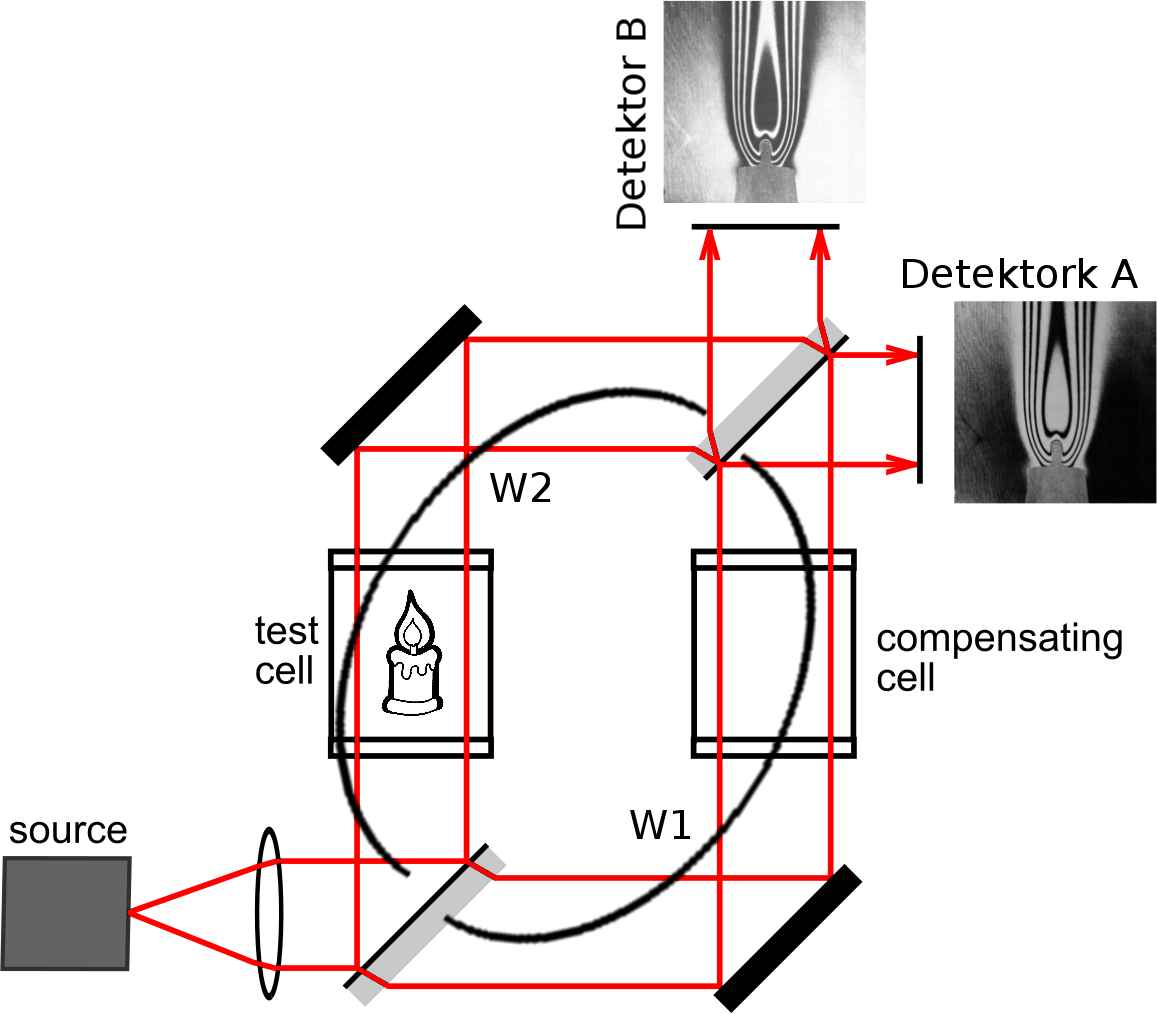
\includegraphics[width=0.7\textwidth]{Mach_Zehnder_interferometer.png}
				\caption{Schematischer Aufbau eines Mach-Zehnder-Interferometers. Ein kollimierter Lichtstrahl (\tilt{source}, Linse) trifft einerseits auf eine Probe (\tilt{test cell}) und andererseits auf eine leere Referenzkammer (\tilt{compensating cell}). Unterschiedliche Interferenzbilder werden auf 2 Schirmen, den Detektoren \fett{A} und \fett{B} nach Überlagerung beobachtet. \cite{WikiMZInt}}
				\label{img:aufbau}
			\end{figure}

\clearpage
			\subsection{MZ-Interferometer für Wellen}

				Nach \autoref{img:aufbau} durchläuft jeweils ein Strahl den Weg \fett{W1} und \fett{W2} mit den Weglängen $s\ix{W1}$ bzw. $s\ix{W2}$. Offensichtlich erfahren beide eine unterschiedliche Phasenverschiebung aufgrund der Probe bzw. den Reflexionen an Spiegeln und dem Durchgang durch die Strahlteiler.\\
				Bei der Reflexion eines Lichtstrahls einem optisch dichteren Medium - unter Annahme einer, zur Einfallsebene senkrecht polarisiert einlaufenden Welle und nicht-absorbierender Medien - tritt \enquote{für die zur Einfallsebene senkrechte Komponente ein Phasensprung von $\pi$ auf.} (aus \cite{MZdemt}, S. 239). Gleiches gilt auch für die Parallelkomponente und jeden Einfallswinkel (exc. den \tilt{Brewster-Winkel}) womit man annehmen kann: \enquote{Die Welle macht dann einen Phasensprung von $\pi$ bei der Reflexion.}\\
				Untersucht man nun die einzelnen Wege des Lichtstrahls - \fett{W1} oder \fett{W2} zum Detektor \fett{A} oder \fett{B} - so findet man, dass der gesamte Phasenunterschied jeweils $2\pi$ beträgt und man somit auf beiden Schirmen konstruktive Interferenz, e.g. \tilt{kohärente} Überlagerung  erwarten muss.\\
				Augenscheinlich muss zusätzlich die, bisher vernachlässigte Richtungsabhängigkeit eines Strahlteilers und der daran stattfindenden Reflexion beachtet werden. Es kommt demnach zu keinem Phasensprung bei einer Reflexion an der 'Rückseite', dem halb-durchlässigen Spiegel eines realen Strahlteilers.\\
				Tatsächlich nimmt eine durchlaufende Welle im Glas des Bauteils eine zusätzliche Phase von $2\pi s/\lambda$ auf, wobei $\lambda$ die Wellenzuglänge und $s$ der optische Weg im Medium - respektive Brechungsindex und Einfallswinkel - ist. Damit wird entlang des Pfades \fett{W1} zum Detektor \fett{A} die Gesamt-Phasenverschiebung zu $\varphi\ix{A}$ in \autoref{eq:phas1a}. Analog gilt dies für den anderen Detektor \fett{B} und den zweiten Pfad \fett{W2} in \autoref{eq:phas1b} - \autoref{eq:phas2b}.

					\begin{align}
						\varphi\ix{A}=&\pi+\pi+\frac{2\pi s}{\lambda}+\frac{2\pi s\ix{W1}}{\lambda} \label{eq:phas1a} \\
						\varphi\ix{B}=&\pi+\pi+\pi+\frac{2\pi s}{\lambda}+\frac{2\pi s\ix{W1}}{\lambda}=\phi\ix{1}+\pi \label{eq:phas1b} \\
						\vartheta\ix{A}=&\pi+\pi+\frac{2\pi s}{\lambda}+\frac{2\pi s\ix{W2}}{\lambda} \label{eq:phas2a} \\
						\vartheta\ix{B}=&\pi+2\frac{2\pi s}{\lambda}+\frac{2\pi s\ix{W2}}{\lambda} \label{eq:phas2b}
					\end{align}

			Mit der Kenntnis über die Phasen-\tilt{shifts} können nun eindeutig Interferenzverhältnisse vorhergesagt werden. Die Differenz aus $\varphi\ix{A}$ und $\vartheta\ix{A}$ entspricht gerade der Phasenrelation zwischen den Wellen entlang der beiden Pfade auf den Detektor \fett{A} in \autoref{eq:phasrel}. Gleiches gilt für die Überlagerung auf Schirm \fett{B} in \autoref{eq:phasrel2} \cite{MZwork}.

				\begin{align}
					\varphi\ix{A}-\vartheta\ix{A}=&\frac{2\pi (s\ix{W1}-s\ix{W2})}{\lambda}=\delta \label{eq:phasrel}\\
					\varphi\ix{B}-\vartheta\ix{B}=&\pi+\delta \label{eq:phasrel2}
				\end{align}


			\subsection{MZ-Interferometer für einzelne Photonen}

	\clearpage
	\section{Durchführung}
	
	\clearpage
	\section{Auswertung}
	
	\clearpage
	\section{Anhang}

\bibliography{all}
\bibliographystyle{natdin}

\end{document}